\documentclass[border=2pt]{standalone}
\usepackage{tikz}
\usetikzlibrary{arrows.meta,positioning,calc,fit,backgrounds,shapes.geometric}
\usepackage{amsmath,amssymb}
\usepackage{times}
\definecolor{ink}{HTML}{243447}
\definecolor{cA}{HTML}{4477AA}
\definecolor{cB}{HTML}{CC6677}
\definecolor{cAu}{HTML}{44AA99}
\definecolor{cS}{HTML}{CCAA33}
\definecolor{grn}{HTML}{228833}
\definecolor{rose}{HTML}{AA3377}
\definecolor{inst}{HTML}{F2E3B3}
\tikzset{
 pap/.style={circle,draw=ink,line width=.6pt,minimum size=15pt,inner sep=0pt,font=\scriptsize\bfseries,text=white},
 aut/.style={rectangle,draw=ink,line width=.6pt,minimum size=13pt,inner sep=0pt,fill=cAu,font=\scriptsize\bfseries,text=white},
 sub/.style={diamond,draw=ink,line width=.6pt,minimum size=17pt,inner sep=0pt,fill=cS,font=\scriptsize\bfseries,text=white},
 gone/.style={draw=ink!35,fill=ink!8,text=ink!40,dashed},
 ed/.style={draw=ink,line width=.7pt},
 msg/.style={-{Stealth[length=4pt]},line width=.9pt,draw=rose},
 ptitle/.style={font=\footnotesize\bfseries,text=ink,anchor=west},
 note/.style={font=\scriptsize,text=ink,align=center},
}

\tikzset{
 est/.style={rectangle,draw=grn,fill=grn!15,line width=.5pt,minimum size=6.5pt,inner sep=0pt},
 fst/.style={circle,fill=rose,inner sep=1.8pt},
 stage/.style={draw=ink!50,rounded corners=3pt,line width=.6pt,minimum width=4.1cm,minimum height=4.3cm,anchor=north west,fill=white},
 stnum/.style={circle,fill=ink,text=white,font=\scriptsize\bfseries,inner sep=1.4pt},
 sname/.style={font=\footnotesize\bfseries,text=ink,anchor=west},
 txt/.style={font=\scriptsize,text=ink,align=center},
 vec/.style={draw=ink,fill=#1,minimum width=4.2pt,minimum height=9pt,inner sep=0pt},
 flow/.style={-{Stealth[length=5pt]},line width=1.2pt,draw=ink!60},
 mp/.style={-{Stealth[length=3.5pt]},grn,line width=.9pt},
 tie/.style={line width=.7pt,draw=rose,{Stealth[length=3pt]}-{Stealth[length=3pt]},shorten <=1pt,shorten >=1pt},
 walk/.style={-{Stealth[length=4pt]},rose,line width=1.4pt},
}
\newcommand{\bars}[5]{% x y n fill label-less
 \foreach \k in {1,...,#3}{\node[vec=#4] at (#1+\k*0.1,#2) {};}}
\newcommand{\running}[1]{
 \node[pap,fill=cA] (#1P1) at (0,0) {P1};
 \node[aut] (#1A7) at (1.2,0.75) {A7};
 \node[sub] (#1S3) at (1.2,-0.8) {S3};
 \node[pap,fill=cB] (#1P9) at (2.4,0) {P9};
 \node[pap,fill=cA] (#1P4) at (2.4,1.5) {P4};
}
\newcommand{\runedges}[2]{\draw[#2] (#1P1)--(#1A7) (#1A7)--(#1P9) (#1A7)--(#1P4) (#1P1)--(#1S3) (#1S3)--(#1P9);}
\begin{document}
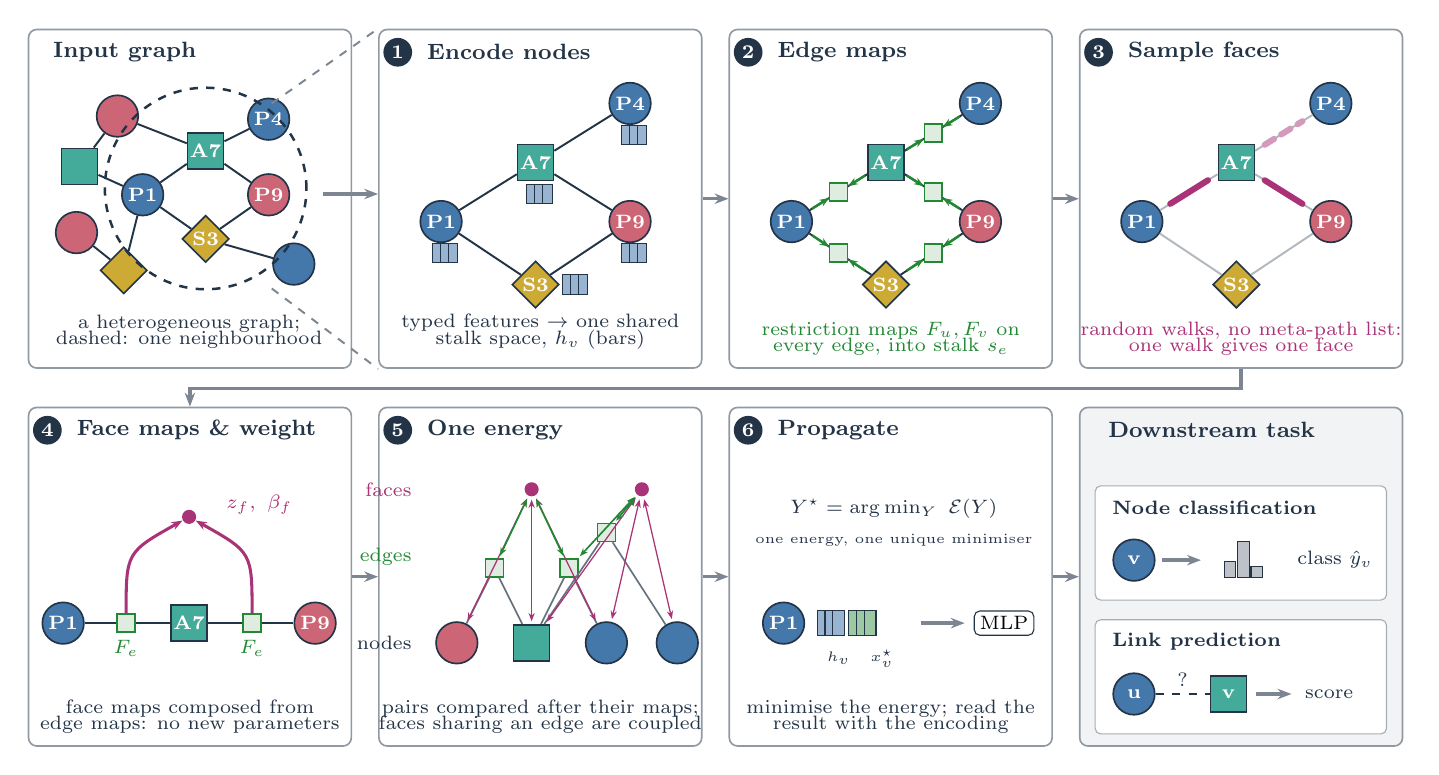
\begin{tikzpicture}
\def\CW{4.45}\def\RH{4.8}
% boxes
\node[stage,minimum width=4.1cm] (BI) at (0,0) {};
\node[sname] at (0.2,-0.3) {Input graph};
\foreach \i/\t in {1/Encode nodes,2/Edge maps,3/Sample faces}{
  \node[stage] (B\i) at (\i*\CW,0) {};
  \node[stnum] at ($(B\i.north west)+(0.25,-0.3)$) {\i};
  \node[sname] at ($(B\i.north west)+(0.5,-0.3)$) {\t};
}
\foreach \i/\t/\c in {4/Face maps \& weight/0,5/One energy/1,6/Propagate/2}{
  \node[stage] (B\i) at (\c*\CW,-\RH) {};
  \node[stnum] at ($(B\i.north west)+(0.25,-0.3)$) {\i};
  \node[sname] at ($(B\i.north west)+(0.5,-0.3)$) {\t};
}
\node[stage,fill=ink!6] (BD) at (3*\CW,-\RH) {};
\node[sname] at ($(BD.north west)+(0.25,-0.3)$) {Downstream task};
% ===== input graph with dashed zoom region
\begin{scope}[shift={(0.5,-0.35)},scale=0.8]
 \node[pap,fill=cA] (iP1) at (1.2,-2.2) {P1};
 \node[aut] (iA7) at (2.2,-1.5) {A7};
 \node[sub] (iS3) at (2.2,-2.9) {S3};
 \node[pap,fill=cB] (iP9) at (3.2,-2.2) {P9};
 \node[pap,fill=cA] (iP4) at (3.2,-1.0) {P4};
 \node[pap,fill=cB] (iP2) at (0.8,-0.95) {};
 \node[aut] (iA2) at (0.2,-1.75) {};
 \node[pap,fill=cA] (iP6) at (3.6,-3.3) {};
 \node[sub] (iS4) at (0.9,-3.4) {};
 \node[pap,fill=cB] (iP7) at (0.15,-2.8) {};
 \draw[ed] (iP1)--(iA7) (iA7)--(iP9) (iA7)--(iP4) (iP1)--(iS3) (iS3)--(iP9)
           (iA2)--(iP2) (iA2)--(iP1) (iS3)--(iP6) (iP2)--(iA7) (iS4)--(iP7) (iS4)--(iP1);
 \draw[ink,dashed,line width=.9pt] (2.2,-2.1) circle (1.6);
\end{scope}
\node[txt] at (2.05,-3.85) {a heterogeneous graph;\\[-2pt]dashed: one neighbourhood};
\draw[dashed,ink!60,line width=.7pt] (3.1,-0.95)--(B1.north west);
\draw[dashed,ink!60,line width=.7pt] (3.1,-3.3)--(B1.south west);
\draw[flow] (3.75,-2.1)--(\CW,-2.1);
% ===== stage 1: encode
\begin{scope}[shift={(\CW+0.8,-2.45)},scale=1.0]
 \running{a} \runedges{a}{ed}
 \foreach \k in {1,2,3}{\node[vec=cA!55,minimum height=7pt,minimum width=3.4pt] at ($(aS3)+(0.3+\k*0.1,0)$) {};}
 \foreach \n in {aP1,aA7,aP9,aP4}{\foreach \k in {1,2,3}{\node[vec=cA!55,minimum height=7pt,minimum width=3.4pt] at ($(\n)+(-0.15+\k*0.1,-0.4)$) {};}}
\end{scope}
\node[txt] at ($(B1.north)+(0,-3.85)$) {typed features $\to$ one shared\\[-2pt]stalk space, $h_v$ (bars)};
% ===== stage 2: edge maps
\begin{scope}[shift={(2*\CW+0.8,-2.45)},scale=1.0]
 \running{b} \runedges{b}{ed}
 \foreach \u/\v in {bP1/bA7,bA7/bP9,bA7/bP4,bP1/bS3,bS3/bP9}{
   \node[est] (m) at ($(\u)!0.5!(\v)$) {};
   \draw[mp] ($(\u)!0.22!(\v)$)--($(\u)!0.40!(\v)$); \draw[mp] ($(\v)!0.22!(\u)$)--($(\v)!0.40!(\u)$);}
\end{scope}

\node[txt,text=grn,anchor=north] at ($(B2.north)+(0,-3.6)$) {restriction maps $F_u,F_v$ on\\[-2pt]every edge, into stalk $s_e$};
% ===== stage 3: sample faces
\begin{scope}[shift={(3*\CW+0.8,-2.45)},scale=1.0]
 \running{c} \runedges{c}{ed,ink!35}
 \draw[rose,line width=2.2pt,line cap=round] ($(cP1)!0.3!(cA7)$)--($(cP1)!0.7!(cA7)$);
 \draw[rose,line width=2.2pt,line cap=round] ($(cA7)!0.3!(cP9)$)--($(cA7)!0.7!(cP9)$);
 \draw[rose!50,line width=2.2pt,line cap=round,dash pattern=on 4pt off 3pt] ($(cA7)!0.3!(cP4)$)--($(cA7)!0.7!(cP4)$);
 \node[rose,font=\scriptsize] at (1.2,1.25) {};
\end{scope}

\node[txt,text=rose,anchor=north] at ($(B3.north)+(0,-3.6)$) {random walks, no meta-path list:\\[-2pt]one walk gives one face};
% ===== stage 4: face maps
\begin{scope}[shift={(0.45,-\RH-2.75)}]
 \node[pap,fill=cA] (dP1) at (0,0) {P1};
 \node[aut] (dA7) at (1.6,0) {A7};
 \node[pap,fill=cB] (dP9) at (3.2,0) {P9};
 \draw[ed] (dP1)--(dA7)--(dP9);
 \node[est] (de1) at (0.8,0) {}; \node[est] (de2) at (2.4,0) {};
 \node[fst] (dz) at (1.6,1.35) {};
 \draw[-{Stealth[length=4pt]},rose,line width=1.1pt] (de1)..controls (0.8,0.9) .. (dz);
 \draw[-{Stealth[length=4pt]},rose,line width=1.1pt] (de2)..controls (2.4,0.9) .. (dz);
 \node[rose,font=\scriptsize,anchor=west] at (1.95,1.5) {$z_f,\ \beta_f$};
 \node[grn,font=\scriptsize] at (0.8,-0.32) {$F_e$}; \node[grn,font=\scriptsize] at (2.4,-0.32) {$F_e$};
\end{scope}

\node[txt,anchor=north] at ($(B4.north)+(0,-3.6)$) {face maps composed from\\[-2pt]edge maps: no new parameters};
% ===== stage 5: energy, three levels
\begin{scope}[shift={(\CW+1.0,-\RH-3.0)}]
 \node[pap,fill=cB] (n9) at (0,0) {}; \node[aut] (n7) at (0.95,0) {}; \node[pap,fill=cA] (n1) at (1.9,0) {}; \node[pap,fill=cA] (n4) at (2.8,0) {};
 \node[est] (e97) at (0.475,0.95) {}; \node[est] (e71) at (1.425,0.95) {}; \node[est] (e74) at (1.9,1.4) {};
 \node[fst] (zf) at (0.95,1.95) {}; \node[fst] (zg) at (2.35,1.95) {};
 \draw[ink!70,line width=.6pt] (n9)--(e97) (n7)--(e97) (n7)--(e71) (n1)--(e71) (n7)--(e74) (n4)--(e74);
 \foreach \n in {n9,n7,n1} \draw[tie,line width=.45pt] (zf)--(\n);
 \foreach \n in {n1,n7,n4} \draw[tie,line width=.45pt] (zg)--(\n);
 \foreach \e in {e97,e71} \draw[tie,grn,line width=.6pt] (zf)--(\e);
 \foreach \e in {e71,e74} \draw[tie,grn,line width=.6pt] (zg)--(\e);
 \node[txt,anchor=east,text=rose] at (-0.45,1.95) {faces};
 \node[txt,anchor=east,text=grn] at (-0.45,1.1) {edges};
 \node[txt,anchor=east] at (-0.45,0.0) {nodes};
\end{scope}
\node[txt,anchor=north] at ($(B5.north)+(0,-3.6)$) {pairs compared after their maps;\\[-2pt]faces sharing an edge are coupled};
% ===== stage 6: propagate
\begin{scope}[shift={(2*\CW+0.25,-\RH-1.3)}]
 \node[txt] at (1.85,0.0) {$Y^\star=\arg\min_Y\ \mathcal{E}(Y)$};
 \node[txt,font=\tiny] at (1.85,-0.4) {one energy, one unique minimiser};
 \node[pap,fill=cA] (p) at (0.45,-1.45) {P1};
 \foreach \k in {1,...,3}{\node[vec=cA!55] at (0.85+\k*0.1,-1.45) {};}
 \foreach \k in {1,...,3}{\node[vec=grn!45] at (1.25+\k*0.1,-1.45) {};}
 \node[txt,font=\tiny] at (1.15,-1.9) {$h_v$}; \node[txt,font=\tiny] at (1.7,-1.9) {$x^\star_v$};
 \draw[flow] (2.2,-1.45)--(2.75,-1.45);
 \node[draw=ink,rounded corners=2pt,fill=white,font=\scriptsize,inner sep=2pt] at (3.25,-1.45) {MLP};
\end{scope}

\node[txt,anchor=north] at ($(B6.north)+(0,-3.6)$) {minimise the energy; read the\\[-2pt]result with the encoding};
% ===== downstream
\begin{scope}[shift={(3*\CW+0.2,-\RH-1.0)}]
 \node[draw=ink!40,rounded corners=2pt,fill=white,minimum width=3.7cm,minimum height=1.45cm,anchor=north west] at (0,0) {};
 \node[txt,anchor=west] at (0.1,-0.28) {\textbf{Node classification}};
 \node[pap,fill=cA] (qv) at (0.5,-0.95) {v};
 \draw[flow] (0.85,-0.95)--(1.35,-0.95);
 \foreach \k/\h in {1/6,2/13,3/4}{\node[vec=ink!30,minimum height=\h pt,anchor=south] at (1.55+\k*0.17,-1.18) {};}
 \node[txt,anchor=west] at (2.45,-0.95) {class $\hat y_v$};
 \begin{scope}[shift={(0,-1.7)}]
 \node[draw=ink!40,rounded corners=2pt,fill=white,minimum width=3.7cm,minimum height=1.45cm,anchor=north west] at (0,0) {};
 \node[txt,anchor=west] at (0.1,-0.28) {\textbf{Link prediction}};
 \node[pap,fill=cA] (lu) at (0.5,-0.95) {u};
 \node[aut] (lv) at (1.7,-0.95) {v};
 \draw[ink,dashed,line width=.8pt] (lu)--(lv) node[midway,above=-1pt,font=\scriptsize]{?};
 \draw[flow] (2.05,-0.95)--(2.5,-0.95);
 \node[txt,anchor=west] at (2.55,-0.95) {score};
 \end{scope}
\end{scope}
% ===== flows
\draw[flow] (B1.east)--(B2.west);
\draw[flow] (B2.east)--(B3.west);
\draw[flow] (B3.south)--++(0,-0.25) -| (B4.north);
\draw[flow] (B4.east)--(B5.west);
\draw[flow] (B5.east)--(B6.west);
\draw[flow] (B6.east)--(BD.west);
\end{tikzpicture}
\end{document}
